\documentclass[12pt]{article}

\usepackage[a4paper, margin=1in]{geometry}
\usepackage{graphicx}
\usepackage[absolute, overlay]{textpos}
\usepackage{fancyhdr}
\usepackage{siunitx}
\usepackage{tikz}
\usepackage{pgfplots}
\usetikzlibrary{decorations.pathmorphing}
\usetikzlibrary{math}
\usetikzlibrary{calc}

\pgfplotsset{compat=1.18}

\pagestyle{fancy} %for footers

\newcommand{\customsubject}{}   
\newcommand{\customtitle}{}

\newcounter{questionpartcounter}                  %Setup for question part counter for a,b,c listing
\renewcommand{\thequestionpartcounter}
{\alph{questionpartcounter}}

\newcounter{questionpartpartcounter}                  %Setup for question part  partcounter for a,b,c listing
\renewcommand{\thequestionpartpartcounter}
{\roman{questionpartcounter}}

\pagestyle{fancy} %for footers
\renewcommand{\headrulewidth}{0pt}
\fancyhf{}
\fancyfoot[R]{\thepage}

\newenvironment{worksheet}[2]
{
    
    \global\renewcommand{\customtitle}{#1}
    \global\renewcommand{\customsubject}{#2}


    \begin{textblock*}{5cm}(0.4cm,0.4cm)
   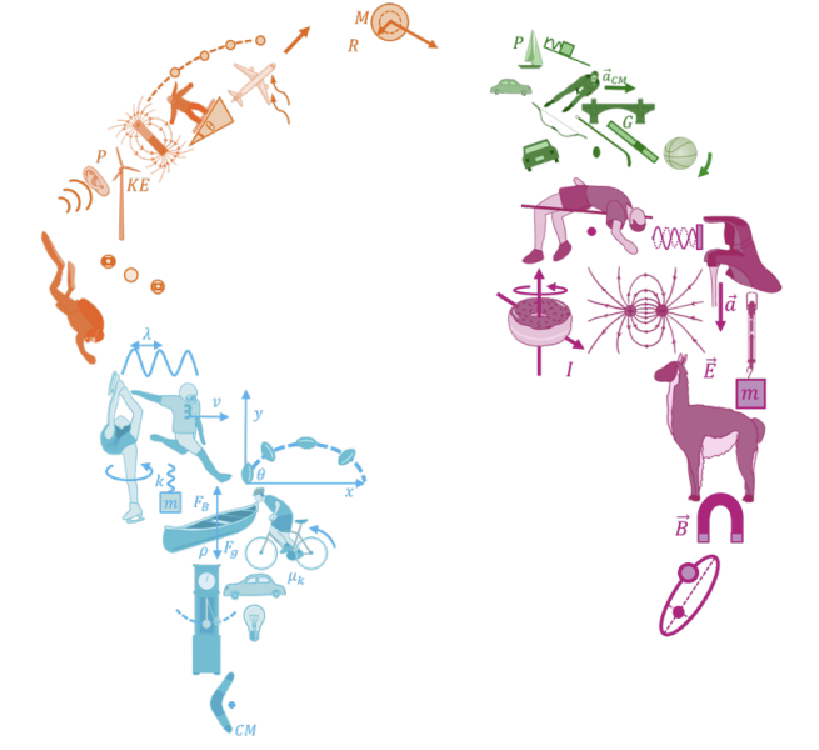
\includegraphics[width=4cm]{include/figures/bmdwlogo}
\end{textblock*}

    \vspace*{-1cm}
    
    {\large\textbf{\begin{center}\customtitle\end{center}}}

    \begin{center}\customsubject\end{center}
    
    \vspace{0.3cm}
    
    \hspace*{-1.5cm}\textbf{Name:\ \rule{4cm}{0.4pt}}\; 
    \textbf{Student \#: \ \rule{3cm}{0.4pt}}\;
    \textbf{Student Email \#: \ \rule{1.53cm}{0.4pt}}

    \vspace{0.5cm}

    
    \begin{enumerate}
}
{
    \end{enumerate}
   % \begin{textblock*}{10cm}(1cm, 28cm) {\footnotesize \scriptsize \customsubject}
    
%\end{textblock*}
}



\newcommand{\question}[2][1cm]{%
    \item
    \setcounter{questionpartcounter}{0}
    \setcounter{questionpartpartcounter}{0}
    {#2}
    \vspace{#1}
}

\newcommand{\questionpart}[2][1cm]{%
    \setcounter{questionpartpartcounter}{0}
    \stepcounter{questionpartcounter}
    (\thequestionpartcounter)~#2
    \vspace{#1}
}

\newcommand{\questionpartpart}[2][1cm]{%
      \stepcounter{questionpartpartcounter}
      \thequestionpartpartcounter.~#2
      \vspace{#1}
}

\newcommand{\operation}[1]{%
{\large $
#1
$}
}



\begin{document}

\begin{worksheet}{Physics Worksheet}{Rotational Energy and Momentum}

\question[3cm]{A hoop, a disk, and a sphere roll without slipping down an incline. If they are all
released at the same time, in what order will they arrive at the bottom? Explain why:}


\question[4cm]{Take an elliptical orbit. Kepler's second law states that: a line from the sun to a planet sweeps out equal areas in equal time intervals. After reading this chapter, what is another way you can express this same concept?}

\question[0.5cm]{Consider a perfect pendulum. What would a Lagrangian look like for the system using angular qualities?}

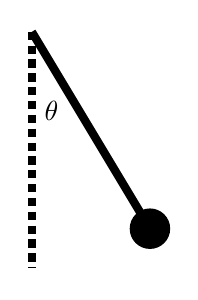
\begin{tikzpicture}
\draw[dotted, line width = 3pt] (0,0)--(0,-3);
\draw[line width = 3pt] (0,0)--(1.5,-2.5);
\draw[fill=black] (1.5,-2.5) circle (0.25cm);
\node at (0.25,-1){$\theta$};


\end{tikzpicture}




\newpage

\question[7cm]{Your friend Atlas, just having finished the rotational dynamics unit, tells you they believe that if you were to throw a ball at the equator, and The Earth and everything else with it disappeared, the ball would go flying off into space at high speeds due because of the speed it got from The Earth's rotation energy. Design a model, estimate, and conclude whether Atlas is correct in their thinking or not.}




\question[0cm]{You are about to start climbing a mountain when a spherical rock suddenly rolls passed you down the mountain (without slipping) with a speed of $\SI{200}{\meter\per\second}$. If the mountain has an average of a $15^\circ$ slope, how tall is it?}






\end{worksheet}


\end{document}